\subsection{Camera Selection for Driver Monitoring Systems (DMS)}

In embedded vision applications, particularly within Driver Monitoring Systems (DMS), the camera serves as the primary sensor, capturing essential visual data for analysis. The selection of an appropriate camera is crucial to ensure accurate monitoring of the driver's face, eyes, and upper body movements. This section outlines key criteria for camera selection to optimize the effectiveness of DMS.

\subsubsection{\textbf{Image Sensor} (CCD vs. CMOS)}


\begin{figure}[!h]
     \centering
     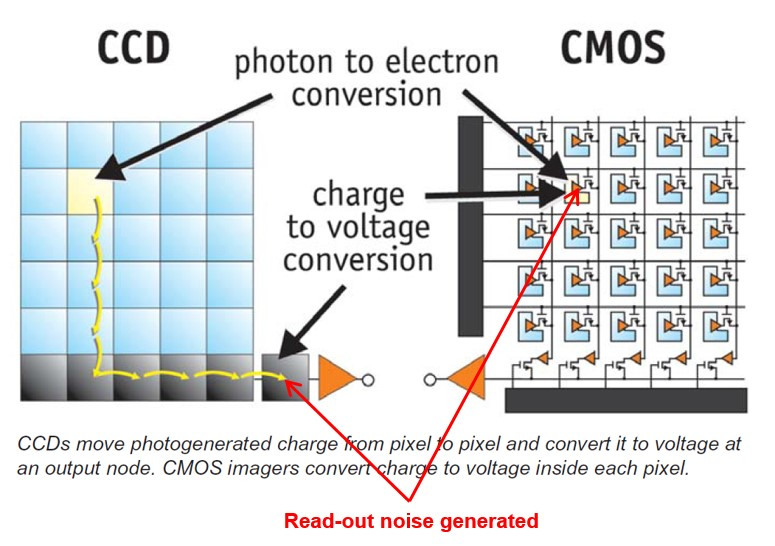
\includegraphics[scale =0.3]{Images/4.1_Camera_Selection/CCDVsCMOS.jpg}
     \caption{CCD vs. CMOS Operation}
     \label{fig:CCDVsCMOS}
\end{figure}

The debate between CCD (Charge-Coupled Device) and CMOS (Complementary Metal-Oxide-Semiconductor) sensors has shaped the evolution of digital cameras, particularly in still photography. As shown in Figure \ref{fig:CCDVsCMOS}, CCD sensors dominated early digital cameras for their superior image quality and specific applications.They operate on a charge-transfer mechanism with a serial process requiring mechanical shutters to prevent smear artifacts during readout. In contrast, CMOS sensors gained prominence with their parallel readout capability, enabling faster processing, lower power consumption, and integration with advanced functionalities like live-view and electronic shutters. Canon's introduction of the first full-frame CMOS sensor in 2002 marked a significant milestone, accompanied by sensor design and manufacturing advancements. Objectively, CCD sensors offer superior image quality with accurate color rendition and smooth tonal transitions but consume more power, generate heat, and have slower readout speeds. CMOS sensors, on the other hand, provide faster readout speeds, lower power consumption, and improved noise performance, particularly in low-light conditions, enhanced further by innovations like Backside Illumination (BSI). Subjectively, while CCD sensors excel in scenarios requiring precise color fidelity and minimal noise at base ISO, CMOS sensors are versatile, supporting high-speed continuous shooting, video recording, and real-time viewing, aligning well with evolving industry demands.

For DMS, CMOS technology is preferred due to its lower power consumption, superior noise performance, and compatibility with real-time video processing, making it ideal for capturing detailed driver behavior effectively.

\subsubsection{\textbf{Shutter Type} (Global Vs. Rolling)}
Exposure time is a period of the shutter from open to close. During the period, the light exposing on the chip’s photosensitive array and Photoelectric effect occurs. After that, photoelectric charges are produced. By the A/D transformation, the value of each pixel is displayed. Under a certain light intensity, the longer the shutter is open, the longer the exposure time, the brighter the image. Long exposure time can show the trajectory of slow moving objects on an image. Short exposure time can record things more accurately. 

In digital cameras, there is usually no mechanical shutter which determines the exposure time. Instead, an electronic shutter is used. This process involves resetting the pixel just before the exposure period starts to return it to its initial state. At the end of the exposure period, the pixel is read out to capture the signal generated by the incident light. Two types of electronic shutters can be used: global shutter and rolling shutter, which differ in their timing mechanisms.

\begin{figure}[!h]
     \centering
     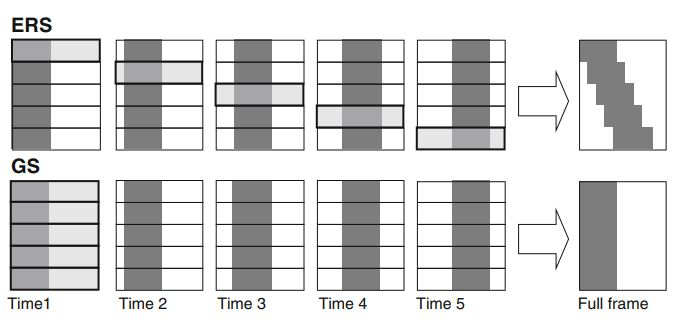
\includegraphics[scale =0.8]{Images/4.1_Camera_Selection/GlobalVsRolling.jpg}
     \caption{Difference of electronic rolling shutter (ERS) and global shutter (GS)}
     \label{fig:GlobalVsRolling}
\end{figure}


As shown in Figure \ref{fig:GlobalVsRolling}, in global shutter mode, each pixel in the sensor begins and ends the exposure simultaneously. This mode requires a significant amount of memory, as the entire image must be stored in memory after the exposure ends and can then be read out gradually. The manufacturing process for global shutter sensors is relatively complex, making them more expensive. However, the advantage of a global shutter is its ability to capture high-speed moving objects without distortion, making it suitable for a wide range of applications.

In rolling shutter mode, different lines of the sensor array are exposed at different times as the readout sweeps through the sensor, as shown in Figure \ref{fig:GlobalVsRolling}. The first line is exposed first, followed by a readout period, then the second line starts exposure, and so on. This sequential exposure means each line reads out before the next line begins. Each pixel in a rolling shutter sensor requires only two transistors to transport electrons, resulting in lower heat production and reduced noise. Compared to global shutter sensors, rolling shutter sensors have a simpler structure and lower cost. However, because each line is not exposed simultaneously, rolling shutters can produce distortion when capturing high-speed moving objects, as shown in figure \ref{fig:GlobalVsRolling2}.

\begin{figure}[!h]
     \centering
     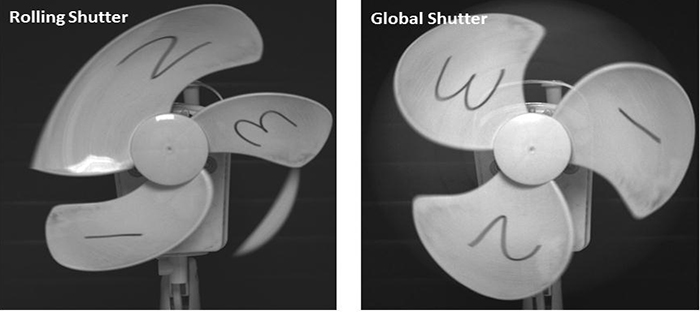
\includegraphics[scale =0.6]{Images/4.1_Camera_Selection/GlobalVsRolling2.jpg}
     \caption{Comparison of rolling and global shutter in high-speed imaging of moving objects}
     \label{fig:GlobalVsRolling2}
\end{figure}

For DMS applications, where accurately capturing the driver's movements and behaviors in real-time is crucial, the global shutter is the preferred choice.



\subsubsection{\textbf{Monochrome vs. Color Camera Modules}}

\textbf{Monochrome Camera Module} \\
Monochrome camera modules capture images exclusively in shades of gray. 

One significant advantage of monochrome cameras is their higher sensitivity to light compared to color cameras. This increased sensitivity is due to the absence of a color filter array, which allows more light to reach the sensor. Consequently, monochrome cameras can capture clearer and sharper images in low-light conditions.

Additionally, monochrome cameras offer higher resolution. Each pixel in a monochrome camera captures all incoming light, whereas each pixel in a color camera captures only one color. This results in monochrome cameras being able to capture more details and produce higher-quality images.

However, a notable limitation of monochrome cameras is their inability to capture color images. If color information is essential for application, a color camera is necessary. Furthermore, monochrome cameras are typically more expensive than color cameras.

\textbf{Color Camera Module} \\
Color camera modules capture images in full color with many types of color filter arrays.

An advantage of color cameras is their ability to capture images in full color, which is crucial for applications requiring color information. Additionally, color cameras are generally more affordable than monochrome cameras, making them popular for consumer applications like smartphones and digital cameras.

Another benefit of color cameras is their ability to capture images at a faster rate. The color filter array in these cameras allows them to capture all three primary colors (red, green, and blue) simultaneously, enabling faster image capture.

However, color cameras have a lower sensitivity to light compared to monochrome cameras. The color filter array reduces the amount of light reaching the sensor, which can result in less sharp and detailed images in low-light conditions.

For applications like DMS, requiring high sensitivity and detailed resolution, especially in low-light conditions, monochrome cameras are preferable.

\subsubsection{\textbf{Protocol and Interface}}

When designing DMS system, selecting the optimal interface for transmitting visual information is critical to its overall performance. This interface serves as the physical connection layer that links the camera to the processing platform, facilitating image transmission and subsequent processing. Key considerations include throughput capabilities and transmission distance.

In response to increasing demands for high-speed connectivity, the market offers a range of flexible and robust interfaces. Among the most widely adopted are MIPI CSI-2, GMSL, and USB interfaces, each tailored to meet specific industry needs

\textbf{MIPI CSI-2}\\ 
MIPI CSI-2, or Mobile Industry Processor Interface Camera Serial Interface Type-2, is a high-speed serial interface primarily developed for transmitting image and video data from mobile camera modules to embedded processors. Originally designed for mobile devices, MIPI CSI-2 has found widespread adoption in mobile phones, tablets, and handheld embedded systems due to its versatility and performance capabilities.

The interface supports a peak bandwidth of 6 Gbps, with a practical bandwidth typically around 5 Gbps. It utilizes four image data lanes, each capable of transmitting up to 1.5 Gbps, surpassing the speed of USB 3.0. MIPI CSI-2 is renowned for its efficiency and reliability, capable of handling video resolutions ranging from 1080p to 8K and beyond. It also minimizes CPU resource consumption, leveraging the capabilities of multi-core processors.

MIPI CSI-2 is designed with low power consumption in mind, making it well-suited for battery-powered embedded devices. Its scalability, enabled by multiple data lanes, allows for flexible adjustment of data transfer rates based on application requirements. The interface employs a differential signaling scheme, enhancing noise immunity and ensuring high reliability in data transmission.

However, MIPI CSI-2 has limitations, including a maximum supported cable length of 30 cm, which restricts its use over longer distances. Additionally, implementing MIPI CSI-2 requires specialized components, potentially increasing the cost of the embedded system.

\textbf{USB} \\
USB (Universal Serial Bus) is a widely adopted data transfer protocol in computing devices and embedded systems. In embedded vision systems, USB 2.0 and 3.0 protocols serve as common interfaces for transferring image and video data from camera sensors to host processors.

USB 2.0 supports a maximum data transfer rate of 480 Mbps, while USB 3.0 significantly increases this bandwidth to 5 Gbps. These interfaces are extensively utilized in embedded vision applications such as surveillance systems, industrial inspection, and machine vision, particularly favored for their low-cost and low-power attributes.

The plug-and-play capability is a notable advantage of USB camera interfaces, simplifying integration and reducing development costs. USB 3.0, with its higher bandwidth of up to 360 MB/s, aligns well with the USB3 Vision Standard in embedded vision systems, facilitating seamless device replacement and enhancing flexibility.

However, USB interfaces have limitations. Both USB 2.0 and 3.0 support a maximum cable length of 5 meters, which can restrict deployment options. Additionally, these interfaces lack dedicated video streaming capabilities, potentially causing delays or loss of image data during transmission.\\

\textbf{GMSL} \\
Gigabit Multimedia Serial Link (GMSL) is a high-speed serial link protocol designed primarily for transmitting image and video data in embedded vision systems, particularly in automotive applications. GMSL enables the transmission of high-speed video, bidirectional control data, and power over a single coaxial cable, supporting distances of up to 15 meters with low latency and high frame rates.

GMSL utilizes differential pair transmission for enhanced noise immunity and data integrity. Its unique encoding scheme reduces electromagnetic interference (EMI), allowing for longer cable lengths and higher data rates compared to traditional serial link interfaces.

Commonly used in ADAS (advanced driver assistance systems), autonomous vehicles, and quality control systems, GMSL is favored for its high bandwidth, reliability, and suitability for long-distance transmission.

However, GMSL interfaces tend to be more expensive than alternatives like USB due to the specialized hardware and software required. Additionally, the protocol's complexity may pose challenges for users unfamiliar with its implementation.\\

In our project, we have chosen MIPI CSI-2 as the interface for transmitting visual information due to its compelling advantages in affordability and reliability. MIPI CSI-2 offers high-speed data transfer capabilities, making it well-suited for handling high-resolution video streams efficiently. Its low power consumption is crucial for our battery-powered application, ensuring extended operational lifetimes without compromising performance.

While MIPI CSI-2 excels in these areas, it's worth noting its limitations compared to USB and GMSL interfaces. Specifically, MIPI CSI-2 supports shorter cable distances compared to USB's 5-meter limit and GMSL's ability to extend up to 15 meters. This constraint may impact flexibility in our system setup but is outweighed by MIPI CSI-2's overall suitability for our application's needs.
